\documentclass[12pt]{beamer}
\usetheme{Madrid}
\usepackage{cmap}
\usepackage[utf8]{inputenc}
\usepackage[czech]{babel}
\usepackage[T1]{fontenc}
\usepackage{hyperref}
\usepackage{amsmath}
\usepackage{amsfonts}
\usepackage{amssymb}
\usepackage{graphicx}
\author[Tým 066, varianta II]{{\Large Tým 066, varianta II\\}Roman Ondráček (xondra58)\\František Jeřábek (xjerab25)\\Pavel Raur (xraurp00)\\ Radim Lipka (xlipka02)}
\title{Překladač jatyka IFJ19}
%\setbeamercovered{transparent} 
%\setbeamertemplate{navigation symbols}{} 
%\logo{} 
%\institute[]{Fakulta informačních technologií VUT}
%\date{} 
%\subject{} 
\begin{document}

\begin{frame}
\titlepage
\end{frame}

\begin{frame}{Obsah prezentace}
\tableofcontents
\end{frame}

\section{Lexikální analýza}
\begin{frame}{Lexikální analýza}
\minipage{0.5\textwidth}
\begin{itemize}
\item Pro odsazení je použit zásobníkový automat.
\end{itemize}
\endminipage
\minipage{0.5\textwidth}
\begin{figure}[!htbp]
    \centering
    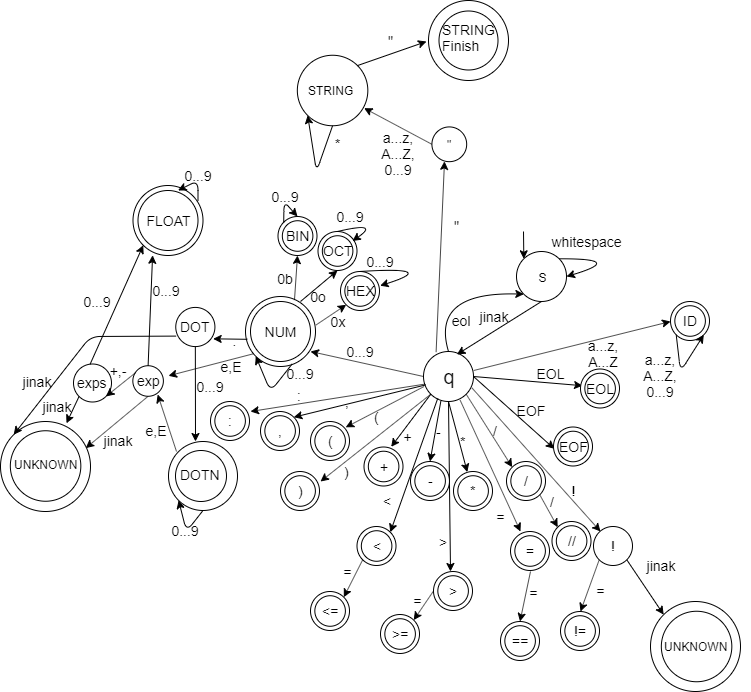
\includegraphics[width = \textwidth]{img/Lexical_Analysis.png}
\end{figure}
 \endminipage
\end{frame}

\section{Syntaktická analýza}
\begin{frame}{Syntaktická analýza}
\begin{itemize}
\item Je použita metoda rekurzivního sestupu.
\item Příkazy jsou složeny z bloků kódu, výrazů, atd.
\item Příkazy jsou určovány podle následujícího tokenu.
\item Během analýzy se plní tabulka symbolů - při definici/volání funkce nebo při přiřazení.
\end{itemize}
\end{frame}

\section{Precedenční syntaktická analýza}
\begin{frame}{Precedenční syntaktická analýza}
\begin{itemize}
\item Je použita pro zpracování výrazů.
\item Je zde použit zásobník podstromů.
\end{itemize}
\begin{table}[!htbp]
\centering
    \begin{tabular}{l l l}
         E $\rightarrow id$ & E $\rightarrow$ E $+$ E & E $\rightarrow$ E $<$ E \\
         E $\rightarrow $ (E) & E $\rightarrow$ E $-$ E & E $\rightarrow$ E $>$ E \\
         E $\rightarrow id$() & E $\rightarrow$ E $*$ E & E $\rightarrow$ E $<=$ E \\
         E $\rightarrow id$(E) & E $\rightarrow$ E $/$ E & E $\rightarrow$ E $>=$ E \\
         E $\rightarrow id$(E, ...) & E $\rightarrow$ E $//$ E & E $\rightarrow$ E $and$ E \\
         E $\rightarrow$ E $==$ E & E $\rightarrow$ E $!=$ E & E $\rightarrow$ E $or$ E \\
         E $\rightarrow not$ E & &  \\
    \end{tabular}
    \caption{Redukční pravidla}
    \label{tab:2}
\end{table}
\end{frame}

\section{Tabulka symbolů}
\begin{frame}{Tabulka symbolů}
\begin{itemize}
\item Implementována pomocí tabulky s rozptýlenými položkami
\item Použitá rozptylovací funkce: \emph{ELF hash}
\item Implementuje část sémantické analýzy - kontroluje počet parametrů funkcí a vícenásobnou definici symbolů
\end{itemize}
\end{frame}

\section{Sémantická analýza}
\begin{frame}{Sémantická analýza}
\begin{itemize}
\item Rekurzivně prochází abstraktní syntaktický strom.
\item Provází implicitní přetypování datových typů.
\item Provádí kontrolu typové kompatibility ve výrazech.
\item Provádí kontrolu, zda do použitých proměnných bylo již přiřazeno.
\end{itemize}
\end{frame}

\section{Generátor tříadresného kódu}
\begin{frame}{Generátor tříadresného kódu}
\begin{itemize}
\item Práce s výrazy.
\item Přiřazení konstant a výrazů.
\item Skoro všechny vestavěné funkce jsou definovány.
\item Bohužel není dokončen. % Máme to vůbec říkat?
\end{itemize}
\end{frame}

\section{Pomocné struktury}
\begin{frame}{Pomocné struktury}
\begin{itemize}
\item Dynamický řetězec
\item Dvousměrně vázaný seznam dynamických řetězců
\item Zásobník pro odsazení
\item Zásobník tokenů
\item Zásobník abstraktních syntaktických stromů
\item Abstraktní syntaktický strom
\end{itemize}
\end{frame}

\begin{frame}{Závěr}
\begin{center}
    \begin{huge}
    Děkujeme za pozornost. \\[8mm]
    \end{huge}
    \large{Dotazy?}
  \end{center}
\end{frame}

\end{document}